\documentclass[11pt, a4paper]{article}
\usepackage[utf8]{inputenc} 
\usepackage[left=2cm,text={17cm, 24cm},top=3cm]{geometry}
\usepackage[czech]{babel}
\usepackage{graphicx}



\begin{document}
	
	\begin{titlepage}
		\begin{center}
			 \textsc{{\Huge Vysoké učení technické v Brně}\\ 
			 \vspace{8.5pt}{\huge Fakulta informačních technologií}}\\
			\vspace{\stretch{0.382}}
			{\LARGE Formální jazyky a překladače\\}
				\vspace{5pt}{\Huge Dokumentace ke skupinovému projektu}\\
				\vspace{2pt}{\Large Tým 47, varianta I}
			\vspace{\stretch{0.618}}\\
		\end{center}
		Jakub Zich (vedoucí) - 25\% \emph{xzichj00} \hfill \\
		Patrícia Hudecová - 25\% \emph{xhudec30} \hfill \\
		Ondřej Marek - 25\% \emph{xmarek67} \hfill\\
		Tomáš Willaschek - 25\% \emph{xwilla00} \hfill
	
	\end{titlepage}	
	\section{Struktura projektu}
	
	\subsection{Lexikální analyzátor}
	\subsection{Syntaktický analyzátor}
	Syntaktický analyzátor (dále jen SA) pracuje na základě trojrozměrného pole, které reprezentuje LL-gramatiku[\ref{ll}]. První rozměr jsou jednotlivé neterminály, druhý všechny možné pravidla pro jeden neterminál a třetí je jedno pravidlo vložené do pole.
	
		Tyto pravidla se aplikují od zadu na zásobník. Aplikace je prováděna dle precedenční analýzy shora dolů - neterminál na vrcholu zásobníku se rozloží podle terminálu na vstupu. 
		
		SA získává tokeny (terminály) voláním lexikálního analyzátoru. Token se následně porovná s vrcholem zásobníku a když se čísla nerovnají, jedná se o syntaktickou chybu.
		
		Tato konkrétní SA musí rozpoznávat, zda je daný výraz funkce, či skutečný výraz. Proto je objem praviděl poněkud rozsáhlejší. 
		
		Kdykoli, když mý být zpracován výraz, volá se spaciální funkce obsažaná přímo v SA, která konvertuje jednotlivé tokeny na dohodnutý string, který následně pošle precedenční analýze ke skontrolování. 
		Kód se ukládá token po tokenu do struktury, která následně slouží pro kontrolu sémantiky a generování kódu. Při získání tokenu EOL se zkontroluje sémantika aktuálního řádku, a pokud je správná, spustí se generování kódu.
		\begin{figure}
			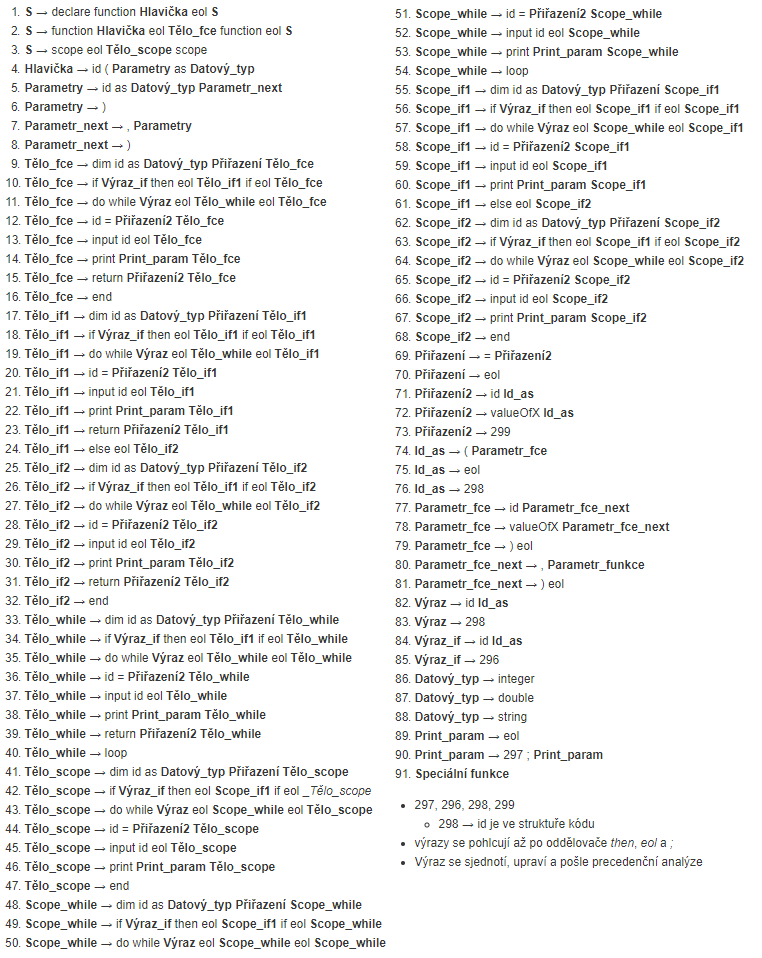
\includegraphics[width=0.999\textwidth]{img/ll.eps}
			\caption{LL-gramatika}
			\label{ll}
		\end{figure}
		\begin{table}[h]
			\centering
			{\scriptsize {\renewcommand{\arraystretch}{1.2}
			\addtolength{\tabcolsep}{-1.1pt}
			\begin{tabular}{|c|c|c|c|c|c|c|c|c|c|c|c|c|c|c|c|c|c|c|c|c|c|c|}
				\hline
				& D & F & S & id & )  & ,  & dim & if & do & I & P & R & end & E & L & =  & eol & V & int & str & dbl & (  \\ \hline
				S                   & 1       & 2        & 3     &    &    &    &     &    &    &       &       &        &     &      &      &    &     &         &         &        &        &    \\ \hline
				Hlavička            &         &          &       & 4  &    &    &     &    &    &       &       &        &     &      &      &    &     &         &         &        &        &    \\ \hline
				Parametry           &         &          &       & 5  & 6  &    &     &    &    &       &       &        &     &      &      &    &     &         &         &        &        &    \\ \hline
				Parametr\_next      &         &          &       &    & 8  & 7  &     &    &    &       &       &        &     &      &      &    &     &         &         &        &        &    \\ \hline
				Tělo\_fce           &         &          &       & 12 &    &    & 9   & 10 & 11 & 13    & 14    & 15     & 16  &      &      &    &     &         &         &        &        &    \\ \hline
				Tělo\_if1           &         &          &       & 20 &    &    & 17  & 18 & 19 & 21    & 22    & 23     &     & 24   &      &    &     &         &         &        &        &    \\ \hline
				Tělo\_if2           &         &          &       & 28 &    &    & 25  & 26 & 27 & 29    & 30    & 31     & 32  &      &      &    &     &         &         &        &        &    \\ \hline
				Tělo\_while         &         &          &       & 36 &    &    & 33  & 34 & 35 & 37    & 38    & 39     &     &      & 40   &    &     &         &         &        &        &    \\ \hline
				Tělo\_scope         &         &          &       & 44 &    &    & 41  & 42 & 43 & 45    & 46    &        & 47  &      &      &    &     &         &         &        &        &    \\ \hline
				Scope\_while        &         &          &       & 51 &    &    & 48  & 49 & 50 & 52    & 53    &        &     &      & 54   &    &     &         &         &        &        &    \\ \hline
				Scope\_if1          &         &          &       & 58 &    &    & 55  & 56 & 57 & 59    & 60    &        &     & 61   &      &    &     &         &         &        &        &    \\ \hline
				Scope\_if2          &         &          &       & 65 &    &    & 62  & 63 & 64 & 66    & 67    &        & 68  &      &      &    &     &         &         &        &        &    \\ \hline
				Přiřazení           &         &          &       &    &    &    &     &    &    &       &       &        &     &      &      & 69 & 70  &         &         &        &        &    \\ \hline
				Přiřazení2          &         &          &       & 71 &    &    &     &    &    &       &       &        &     &      &      &    &     & 72      &         &        &        &    \\ \hline
				Id\_as              &         &          &       &    &    &    &     &    &    &       &       &        &     &      &      &    & 75  &         &         &        &        & 74 \\ \hline
				Parametr\_fce       &         &          &       & 77 & 79 &    &     &    &    &       &       &        &     &      &      &    &     & 78      &         &        &        &    \\ \hline
				Parametr\_fce\_next &         &          &       &    & 81 & 80 &     &    &    &       &       &        &     &      &      &    &     &         &         &        &        &    \\ \hline
				Výraz               &         &          &       & 82 &    &    &     &    &    &       &       &        &     &      &      &    &     &         &         &        &        &    \\ \hline
				Výraz\_if           &         &          &       & 84 &    &    &     &    &    &       &       &        &     &      &      &    &     &         &         &        &        &    \\ \hline
				Datový\_typ         &         &          &       &    &    &    &     &    &    &       &       &        &     &      &      &    &     &         & 86      & 87     & 88     &    \\ \hline
				Print\_param        &         &          &       &    &    &    &     &    &    &       &       &        &     &      &      &    & 89  &         &         &        &        &    \\ \hline
				\multicolumn{23}{c}{D = declare | F = function | S = scope | V = valueOfX | I = input | P = print | R = return | E = else | L = loop }
			\end{tabular}
			}}
			\caption{LL tabulka}
			\label{gramatika}
		\end{table}

		
		
	\subsection{Precedenční analýza}
	\subsection{Sémantický analyzátor}
	\subsection{Generátor kódu}


\end{document}
